\documentclass[xcolor=svgnames,9pt,english, aspectratio=169]{beamer}
%\documentclass[xcolor=svgnames,9pt,english, handout, aspectratio=169]{beamer}
\newcommand{\handout}{0}
% Shared template layer for the six decks: theme, beamer layout, and the packages
% every deck needs. Each deck inputs this near the top of its preamble, BEFORE
% ../common/theme.tex (metropolis must be selected before the palette overrides it).
%
% Notation macros and theorem environments are deliberately NOT shared. They
% conflict between the decks, and merging them would silently change symbols
% inside equations:
%   \e          decks 1-2: \bs{\epsilon}      deck 3: \boldsymbol{\eta}
%   \M          decks 1-2: \mb{M}             deck 3: \mathcal{M}
%   \blue       decks 1-2: blue               deck 3: RoyalBlue
%   \indep      different implementations
%   assumption / proposition
%               decks 1-2: own counter        deck 3: shares the theorem counter
%
% Each deck therefore keeps its own notation block. Only the look is unified.

\usetheme{metropolis}
\setbeamertemplate{navigation symbols}{}

% Deck 3's margins; decks 1 and 2 previously used 2em, which at 9pt is ~6.3mm.
\setbeamersize{text margin left=5mm, text margin right=5mm}
\setbeamertemplate{itemize/enumerate body begin}{\leftmargini=1.5em\relax}
\setbeamertemplate{itemize/enumerate subbody begin}{\leftmarginii=1.5em\relax}
\setbeamertemplate{itemize/enumerate subsubbody begin}{\leftmarginiii=1.5em\relax}

\usepackage{xcolor}
\usepackage{colortbl}
\usepackage{amsmath}
\usepackage{amsfonts}
\usepackage{amssymb}
\usepackage{graphicx}
\usepackage{multirow}
\usepackage{listings}
\usepackage{booktabs}
\usepackage{tikz}
\usetikzlibrary{arrows.meta,positioning,decorations.pathreplacing}

% Citations: one bib file at the repository root, Chicago author-date via biblatex-chicago
% (needs biber). Reference frames are generated with \printbibliography; in-text citations
% use \textcite (narrative) and \parencite (parenthetical). The CMS rule prints one to three
% names in full and four or more as "First et al."; \citeshort forces "et al.", \citeall
% prints every name (text/paren/author variants likewise). The override lasts one citation.
\usepackage{csquotes}
\usepackage[authordate,backend=biber,doi=false,url=false,isbn=false,eprint=false,
            maxbibnames=10,compresspages=true,dashed=false]{biblatex-chicago}
\addbibresource{../references.bib}
% Entry size: beamer wraps each part of a biblatex entry in its "bibliography entry author /
% title / location / note" fonts, and metropolis sets those to \normalsize, so \bibfont alone
% does not change the size. The four \setbeamerfont lines in theme.tex set the size that shows.
\renewcommand*{\bibfont}{\scriptsize}
\setlength{\bibitemsep}{0.7em}   % visible air between entries
\setlength{\bibhang}{0.5em}
% The References frame of every deck: \begin{frame}[t,allowframebreaks=1.0] ... \referencelist.
% Beamer's automatic break for this list fires at about two thirds of the frame; the factor
% 1.1 lets it fill the frame. The small negative skip closes the list's top gap.
\newcommand{\referencelist}{\vspace*{-0.6em}\printbibliography[heading=none]}
\newcommand{\citeshort}[1]{\AtNextCitekey{\defcounter{maxnames}{1}}\cite{#1}}
\newcommand{\textciteshort}[1]{\AtNextCitekey{\defcounter{maxnames}{1}}\textcite{#1}}
\newcommand{\parenciteshort}[1]{\AtNextCitekey{\defcounter{maxnames}{1}}\parencite{#1}}
\newcommand{\citeauthorshort}[1]{\AtNextCitekey{\defcounter{maxnames}{1}}\citeauthor{#1}}
\newcommand{\citeall}[1]{\AtNextCitekey{\defcounter{maxnames}{9}}\cite{#1}}
\newcommand{\textciteall}[1]{\AtNextCitekey{\defcounter{maxnames}{9}}\textcite{#1}}
\newcommand{\parenciteall}[1]{\AtNextCitekey{\defcounter{maxnames}{9}}\parencite{#1}}
% PDF metadata: beamer copies the whole \author box into the author field; set it plainly
% once every deck-level \author has run (etoolbox's end-of-preamble hook).
\AtEndPreamble{\hypersetup{pdfauthor={Yiqing Xu}}}
   % theme, layout, packages

\setbeamertemplate{footline}[frame number]{}

\graphicspath{{./figs/}}%
\newcommand{\red}{\textcolor{red}}

\usepackage{epsfig}
% Shared visual system for the six decks: palette, fonts, footline.
% Swap the four colors below to rebrand every deck at once.
\definecolor{SlideRed}{HTML}{9E1B32}
\definecolor{SlideInk}{HTML}{252A34}
\definecolor{SlideBlue}{HTML}{2F6B9A}
\definecolor{SlideMist}{HTML}{F8F3F3}


\setbeamercolor{normal text}{fg=SlideInk,bg=white}
\setbeamercolor{structure}{fg=SlideRed}
\setbeamercolor{alerted text}{fg=SlideRed}
\setbeamercolor{frametitle}{fg=white,bg=SlideRed}
\setbeamercolor{title}{fg=SlideRed}
\setbeamercolor{subtitle}{fg=SlideInk}
\setbeamercolor{block title}{fg=white,bg=SlideRed}
\setbeamercolor{block body}{fg=SlideInk,bg=SlideMist}
\setbeamercolor{section in toc}{fg=SlideRed}

\setbeamerfont{title}{series=\bfseries,size=\Large}
\setbeamerfont{frametitle}{series=\bfseries,size=\large}
\setbeamerfont{block title}{series=\bfseries}
\setbeamertemplate{navigation symbols}{}
\setbeamertemplate{items}[circle]
\setbeamertemplate{blocks}[rounded][shadow=false]
\setbeamertemplate{bibliography item}{}   % no document icons on the References frames
\setbeamertemplate{frametitle continuation}{}
\setbeamertemplate{footline}{%
  \leavevmode\hbox{%
  \begin{beamercolorbox}[wd=.88\paperwidth,ht=2.6ex,dp=1.2ex,leftskip=1.2em]{author in head/foot}%
  \usebeamerfont{author in head/foot}\insertshorttitle
  \end{beamercolorbox}%
  \begin{beamercolorbox}[wd=.12\paperwidth,ht=2.6ex,dp=1.2ex,center]{date in head/foot}%
  \insertframenumber
  \end{beamercolorbox}}}

\newcommand{\slidesource}[1]{\vfill{\scriptsize\color{gray}Source: #1}}
\newcommand{\keyquestion}[1]{\begin{block}{Question}#1\end{block}}


\title{Panel Methods (4): Two-Way Fixed Effects Revisited}
\subtitle{Lectures on Causal Panel Analysis}
\author{Yiqing Xu\\\smallskip Stanford University}
\date{September 2026}

% ---------- notation (deck-local; do not merge across decks) ----------
\newtheorem{assumption}{Assumption}
\newtheorem{iass}{Identification Assumption}
\newcommand{\bs}{\boldsymbol}
\newcommand{\mb}{\mathbf}
\newcommand{\E}{\ensuremath{\mathbb{E}}}
\newcommand{\X}{\ensuremath{\mb{X}}}
\newcommand{\indep}{{\bot\negthickspace\negthickspace\bot}}
\newcommand{\Tset}{\ensuremath{\mathcal{T}}}
\newcommand{\Cset}{\ensuremath{\mathcal{C}}}

\begin{document}

\AtBeginSection[]
{
  \begin{frame}<beamer>
    \frametitle{Outline}
    \tableofcontents[currentsection]
  \end{frame}
}

\begin{frame}
  \titlepage
  \thispagestyle{empty}
  \addtocounter{framenumber}{-1}
\end{frame}

\begin{frame}
  \frametitle{The Six Lectures}
\begin{center}
\begin{tikzpicture}[
  lecture/.style={rounded corners=3pt, draw=SlideRed, thick,
                  minimum height=1.6cm, text width=2.6cm,
                  align=center, inner sep=5pt},
  link/.style={-{Latex[length=2.2mm]}, thick, draw=SlideInk}
]
\node[lecture, fill=SlideMist] (l1) at (0,0)
  {\textbf{1. Parametric panel models}\\[0.25em]
   \footnotesize FE regressions and their assumptions};
\node[lecture, fill=SlideMist] (l2) at (0,-2.9)
  {\textbf{2. Difference-in-differences}\\[0.25em]
   \footnotesize The canonical design and identification};
\node[lecture, fill=SlideMist] (l3) at (3.9,0)
  {\textbf{3. Factorial DID}\\[0.25em]
   \footnotesize When the event affects everyone};
\node[lecture, fill=SlideRed!25, very thick] (l4) at (3.9,-2.9)
  {\textbf{4. TWFE revisited}\\[0.25em]
   \footnotesize What breaks under staggered timing};
\node[lecture, fill=SlideMist] (l5) at (7.8,0)
  {\textbf{5. Modern DID}\\[0.25em]
   \footnotesize Heterogeneity-robust estimators};
\node[lecture, fill=SlideMist] (l6) at (7.8,-2.9)
  {\textbf{6. Synthetic control \& factor models}\\[0.25em]
   \footnotesize Imputing treated counterfactuals};
\draw[link] (l1) -- (l2);
\draw[link] (l2.east) -- ++(0.5,0) |- (l3.west);
\draw[link] (l3) -- (l4);
\draw[link] (l4.east) -- ++(0.5,0) |- (l5.west);
\draw[link] (l5) -- (l6);
\end{tikzpicture}
\end{center}
\end{frame}

\begin{frame}
  \frametitle{Where We Are}
\begin{itemize}[<+->]\itemsep1em
\item Lecture 1: parametric panel models, with FE regressions as the workhorse
\item Lecture 2: DID as a research design, mostly with two groups and fixed treatment timing
\item Lecture 3: factorial DID, extending the design to events that hit every unit
\item In the two-period case, the TWFE estimate \emph{is} the DID estimate, so the two traditions seem interchangeable
\item Today: what happens when we run TWFE regressions on \alert{many periods}, \alert{staggered timing}, and \alert{heterogeneous effects}, which is what applied work actually looks like
\end{itemize}
\end{frame}

\begin{frame}
  \frametitle{Today's Plan}
\begin{itemize}\itemsep1.5em
\item What assumptions do TWFE models rely upon?
\item Three problems
\begin{itemize}
\item Implications for treatment assignment (design)
\item Parallel trends violations
\item The weighting problem
\end{itemize}
\end{itemize}
\bigskip\pause
\keyquestion{When we estimate $Y_{it} = \tau D_{it} + \alpha_i + \xi_t + \varepsilon_{it}$ on a staggered panel, which comparisons is $\hat{\tau}$ actually making?}
\end{frame}

\section{TWFE and Its Assumptions}

\begin{frame}
  \frametitle{DID: A Quick Review}
\begin{itemize}[<+->]\itemsep0.8em
\item Two groups ($\Tset$, $\Cset$), two periods ($t$ and $t'$), fixed treatment timing
\item Functional form:
\begin{equation*}
Y_{it} = \tau_{it} D_{it} + \alpha_i + \xi_t + \varepsilon_{it}
\quad\text{or}\quad
\begin{cases}
Y_{it}(0) = \alpha_i + \xi_t + \varepsilon_{it}\\
Y_{it}(1) = Y_{it}(0) + \tau_{it}
\end{cases}
\end{equation*}
where $\tau_{it}$ is the treatment effect for unit $i$ at time $t$
\item Parallel trends:
$\E[Y_{it'}(0) - Y_{it}(0) \mid i \in \Tset] = \E[Y_{jt'}(0) - Y_{jt}(0) \mid j \in \Cset]$
\item Or equivalently,
$\E[\varepsilon_{it'} - \varepsilon_{it} \mid i \in \Tset] = \E[\varepsilon_{jt'} - \varepsilon_{jt} \mid j \in \Cset]$
\item $ATT = \E[\tau_{it} \mid D_{it} = 1]$ is nonparametrically identified with two periods (or two treatment histories)
\end{itemize}
\end{frame}

\begin{frame}
  \frametitle{DID as a Missing Data Problem}
\begin{itemize}\itemsep0.8em
\item The treated-group untreated potential outcome after treatment is the one cell we never observe:
\end{itemize}
\begin{center}
\renewcommand{\arraystretch}{1.4}
\begin{tabular}{lcc}
 & Pre & Post \\ \hline
Treated ($\Tset$) & $Y^0_{\Tset,\,pre}$ & \alert{??} \\
Comparison ($\Cset$) & $Y^0_{\Cset,\,pre}$ & $Y^0_{\Cset,\,post}$ \\ \hline
\end{tabular}
\end{center}
\bigskip\pause
\begin{itemize}\itemsep0.8em
\item Parallel trends fills in the missing cell: take the treated pre-period level and add the comparison group's change
\item Every estimator in these lectures is a different rule for filling in that cell
\end{itemize}
\end{frame}

\begin{frame}
  \frametitle{Beyond Two Periods: Block Assignment}
\begin{center}
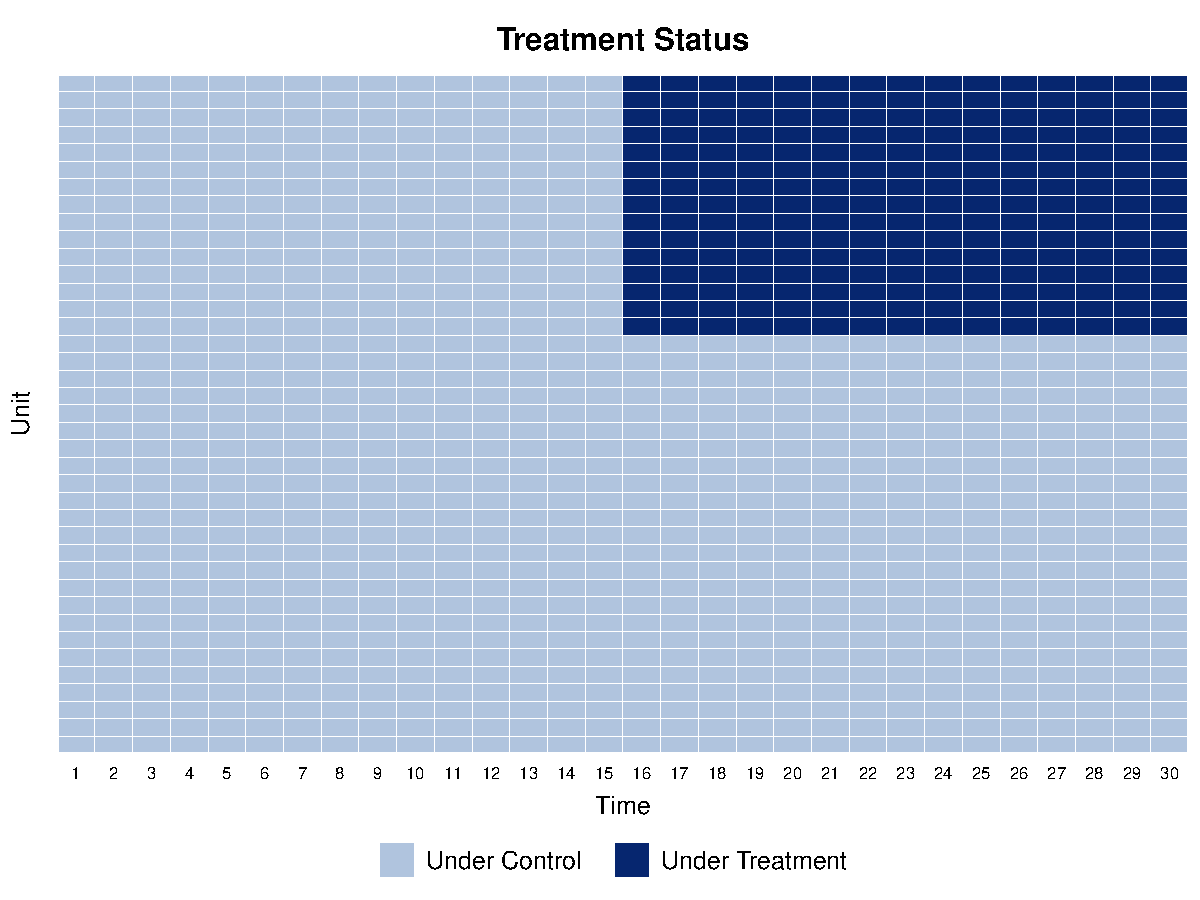
\includegraphics[height=0.68\textheight, keepaspectratio=1]{sim_treat_did.pdf}
\end{center}
\begin{itemize}
\item One adoption date, many periods: still essentially a $2\times 2$ comparison
\end{itemize}
\end{frame}

\begin{frame}
  \frametitle{Beyond Two Periods: Staggered Adoption}
\begin{center}
\if\handout1
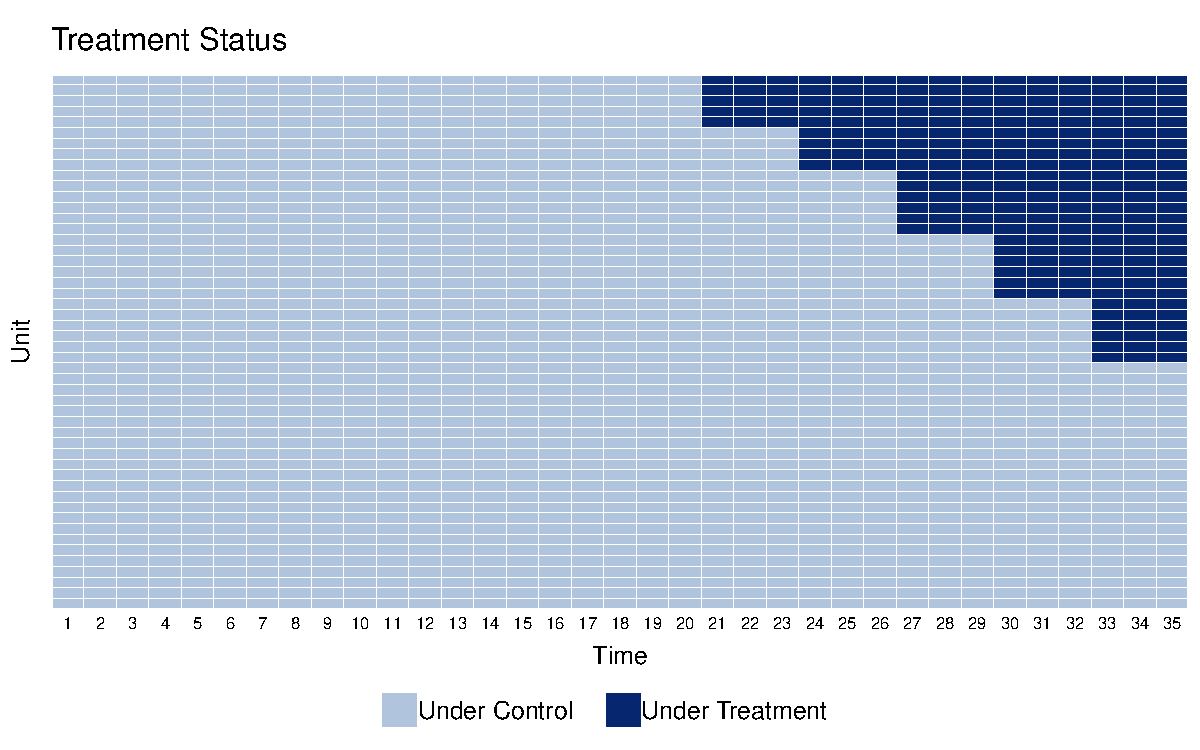
\includegraphics[height=0.68\textheight, keepaspectratio=1]{sim_treat1.pdf}%
\fi
\if\handout0
\only<1>{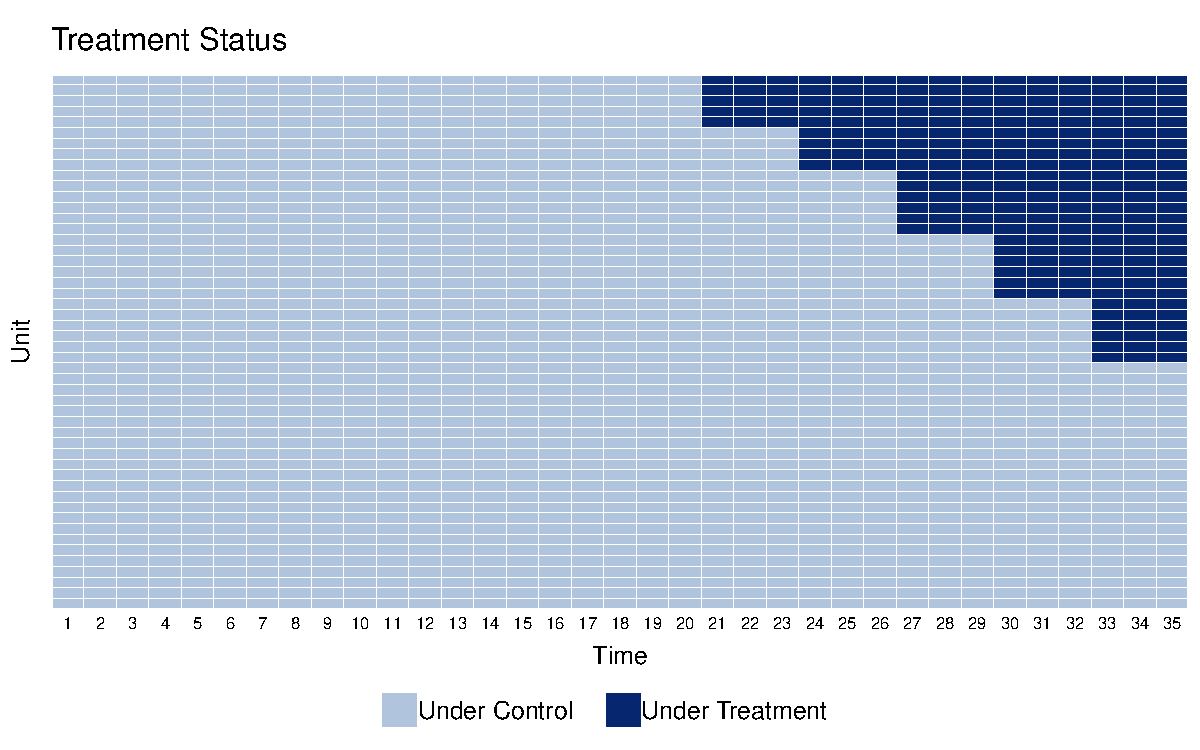
\includegraphics[height=0.68\textheight, keepaspectratio=1]{sim_treat1.pdf}}%
\only<2>{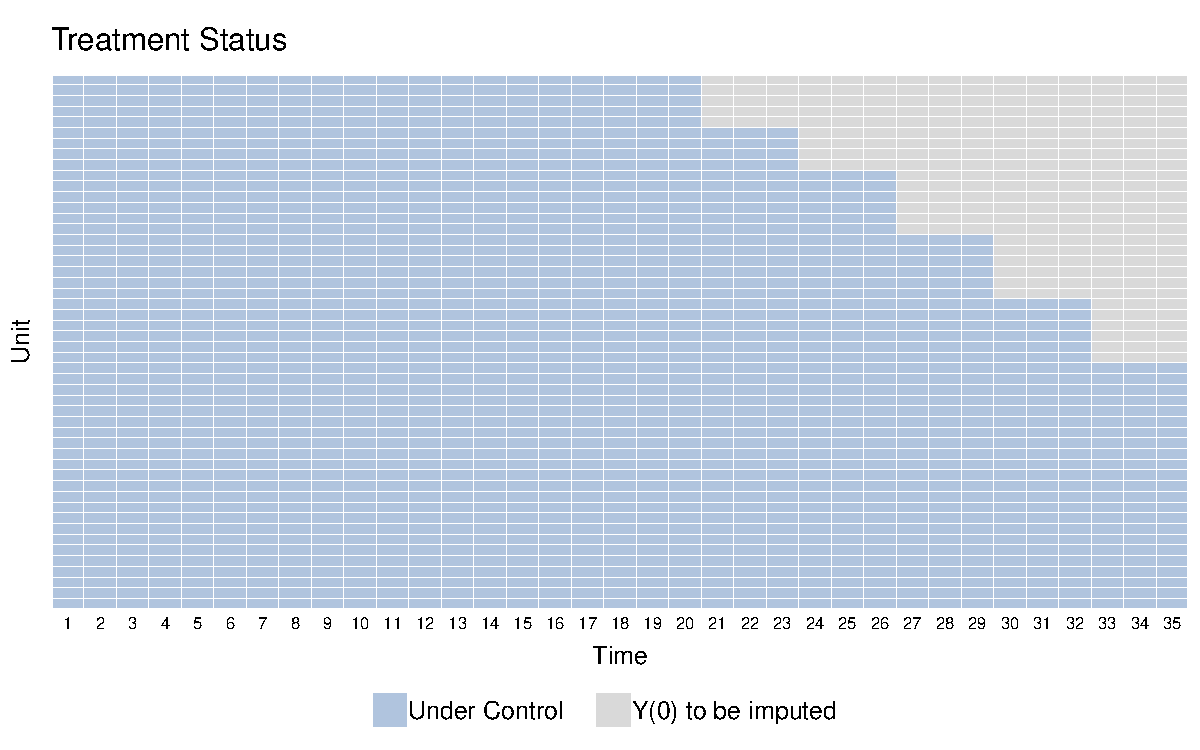
\includegraphics[height=0.68\textheight, keepaspectratio=1]{sim_treat2.pdf}}%
\fi
\end{center}
\begin{itemize}
\item<2-> Different units adopt at different times: the classic staggered setting
\end{itemize}
\end{frame}

\begin{frame}
  \frametitle{Beyond Two Periods: The General Case (with Treatment Reversal)}
\begin{center}
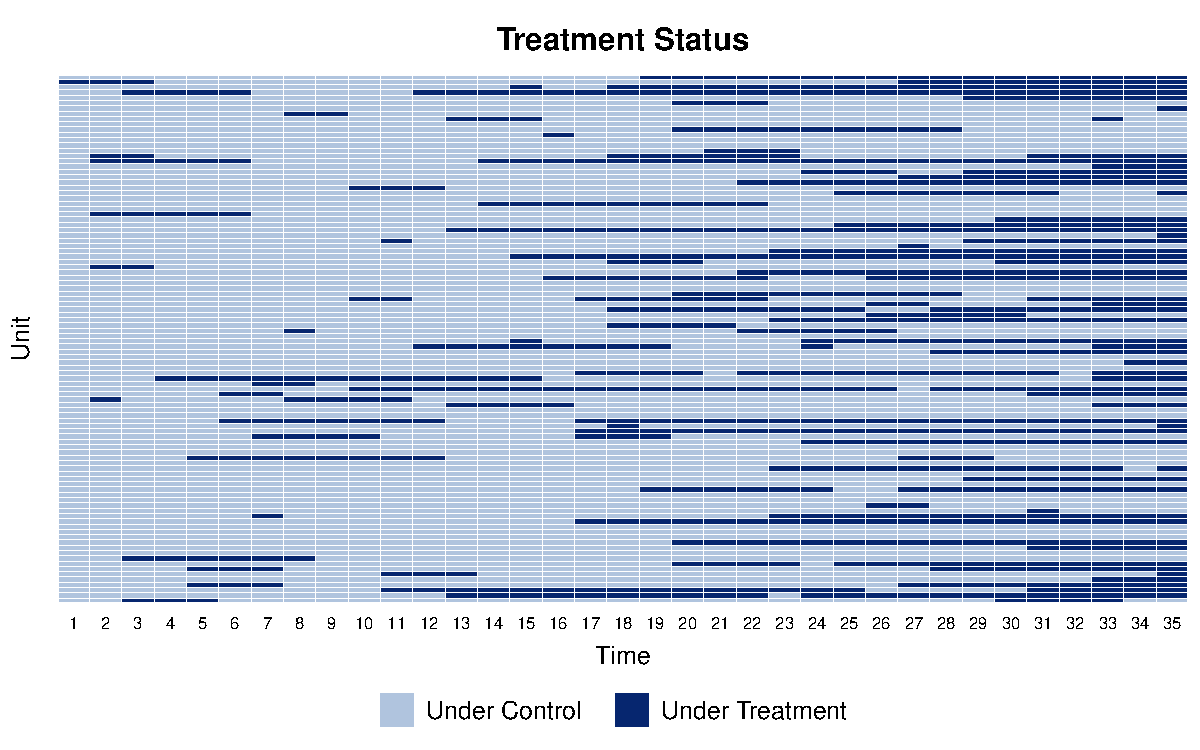
\includegraphics[height=0.68\textheight, keepaspectratio=1]{sim_treat_general.pdf}
\end{center}
\begin{itemize}
\item Treatment can also switch off; the majority of political science applications look like this (we return to it in Lecture 5)
\end{itemize}
\end{frame}

\begin{frame}
  \frametitle{Assumptions for TWFE}
\begin{equation*}
Y_{it} = \tau D_{it} + \X_{it}'\bs{\beta} + \alpha_i + \xi_t + \varepsilon_{it},
\quad D_{it} \in \{0,1\}
\end{equation*}
\bigskip
\begin{itemize}[<+->]\itemsep1em
\item \textbf{Functional form}
\begin{itemize}\itemsep0.4em
  \item Additive fixed effects
  \item \alert{Constant} and contemporaneous treatment effect
  \item Linearity in covariates
\end{itemize}
\item Note the difference from the DID setup: DID allowed $\tau_{it}$ to vary; the TWFE regression assumes a single $\tau$
\item[$\Rightarrow$] When effects are actually heterogeneous, this assumption fails and induces the \alert{(negative) weighting} problem
\end{itemize}
\end{frame}

\begin{frame}
  \frametitle{Assumptions for TWFE: Strict Exogeneity}
\begin{itemize}[<+->]\itemsep1em
\item \textbf{Strict exogeneity}:
\begin{equation*}
\varepsilon_{it} \indep D_{js}, \X_{js}, \alpha_j, \xi_s \qquad \forall\, i, j, t, s
\end{equation*}
\item Which implies
\begin{equation*}
\{Y_{it}(0), Y_{it}(1)\} \indep D_{js} \mid \X, \bs{\alpha}, \bs{\xi} \qquad \forall\, i, j, t, s
\end{equation*}
\item With only two groups, this delivers parallel trends:
\begin{equation*}
\E[Y_{it}(0) - Y_{it'}(0) \mid \X] = \E[Y_{jt}(0) - Y_{jt'}(0) \mid \X], \quad i \in \Tset,\; j \in \Cset,\; \forall\, t, t'
\end{equation*}
\end{itemize}
\end{frame}

\begin{frame}
  \frametitle{Shortcomings of TWFE}
\begin{equation*}
Y_{it} = \tau D_{it} + \X_{it}'\bs{\beta} + \alpha_i + \xi_t + \varepsilon_{it}
\end{equation*}
\bigskip
\begin{itemize}[<+->]\itemsep1em
\item Assumptions
\begin{itemize}\itemsep0.4em
  \item Functional form
  \item Strict exogeneity
\end{itemize}
\item Challenges
\begin{itemize}\itemsep0.4em
  \item Strict exogeneity means a lot more than you think
  \item Prevalent parallel trends failures
  \item Treatment effect heterogeneity leads to bias
\end{itemize}
\end{itemize}
\bigskip
\onslide<8->{We take the three in turn: the design problem, then parallel trends, then weighting.}
\end{frame}

\section{The Design Problem}

\begin{frame}
  \frametitle{Strict Exogeneity Means More Than You Think}
Reinterpreting strict exogeneity (\alert{\cite{imai2019when}}):
\begin{center}
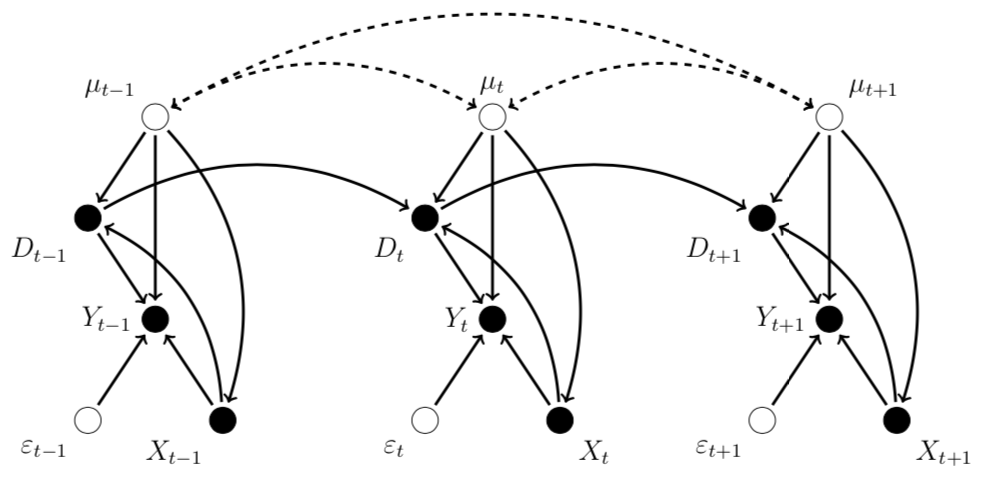
\includegraphics[width=0.44\textwidth]{dag_clean.png}
\end{center}\vspace{-0.6em}\pause
\begin{enumerate}[<+->]\itemsep0.3em
\item No unobserved \alert{time-varying} confounder exists
\item No lagged dependent variable $\rightarrow$ adding an LDV is fine if $T$ is large; not adding it is also fine
\item No ``carryover effect'' $\rightarrow$ adding lagged treatment terms is fine
\item Past outcomes do not directly affect current treatment (no ``feedback'')
\end{enumerate}
\medskip
\onslide<6->{Each of these is a substantive claim about the world, not a regression option.}
\vspace{0.5em}
\end{frame}

\begin{frame}
  \frametitle{Hypothetical Experiment?}
DGPs consistent with \underline{strict exogeneity}:
\begin{center}
$\alpha_{i}, \pmb{X_{i}}$ \pause $\rightarrow \pmb{D_{i}}$ \pause $\rightarrow \pmb{Y_{i}}$\pause
\end{center}
Treatment status is assigned randomly or in one shot, not \underline{sequentially}! \\\medskip\pause
Examples: \red{random assignment} within units\\\pause
\centering
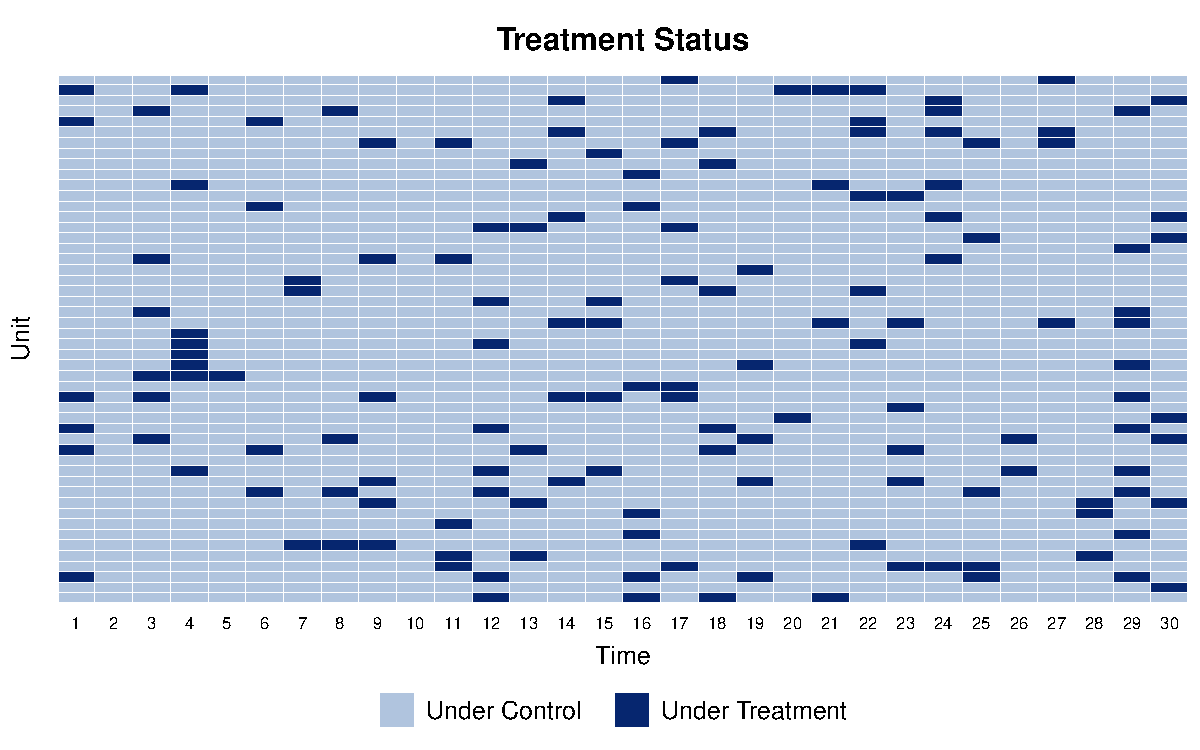
\includegraphics[width=0.6\textwidth, height=0.55\textheight, keepaspectratio]{sim_treat_random.pdf}
\end{frame}

\begin{frame}
  \frametitle{Hypothetical Experiment?}
DGPs consistent with \underline{strict exogeneity}:
\begin{center}
$\alpha_{i}, \pmb{X_{i}}$  $\rightarrow A_{i} \rightarrow \pmb{D_{i}}$ $\rightarrow \pmb{Y_{i}}$
\end{center}
Treatment status is assigned randomly or in one shot, not \underline{sequentially}! \\\medskip
Examples: \red{staggered adoption}, with $A_i$ the adoption time {\small\alert{\parencite{athey2022design}}}\\
\centering
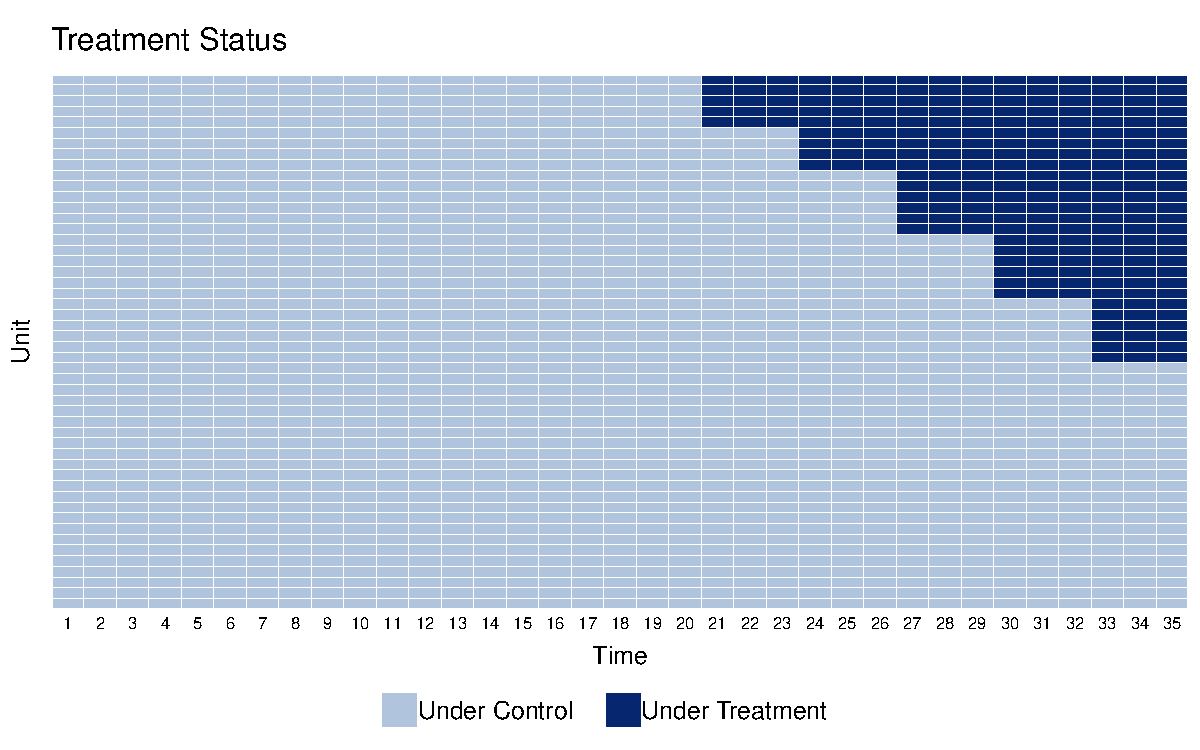
\includegraphics[width=0.6\textwidth, height=0.55\textheight, keepaspectratio]{sim_treat1.pdf}
\end{frame}

\section{Parallel Trends Violations}

\begin{frame}
  \frametitle{The Event-Study (Dynamic TWFE) Specification}
\begin{itemize}[<+->]\itemsep0.9em
\item To probe parallel trends and trace dynamics, applied work estimates
\begin{equation*}
Y_{it} = \sum_{s \neq -1} \mu_s\, \mathbf{1}\{t - T_i = s\} + \alpha_i + \xi_t + \varepsilon_{it}
\end{equation*}
where $T_i$ is unit $i$'s adoption date and $s$ counts periods relative to adoption
\item The period just before adoption ($s = -1$) is the omitted reference category
\item \alert{Leads} ($s < -1$) probe pre-treatment differences; \alert{lags} ($s \geq 0$) trace the dynamic effects
\item Endpoints are usually binned (e.g. $s \leq -8$, $s \geq 12$) so each coefficient rests on enough observations
\end{itemize}
\end{frame}

\begin{frame}
  \frametitle{Failure of Parallel Trends Is Common (1)}
\begin{columns}[T,onlytextwidth]
\begin{column}{0.49\textwidth}
\centering
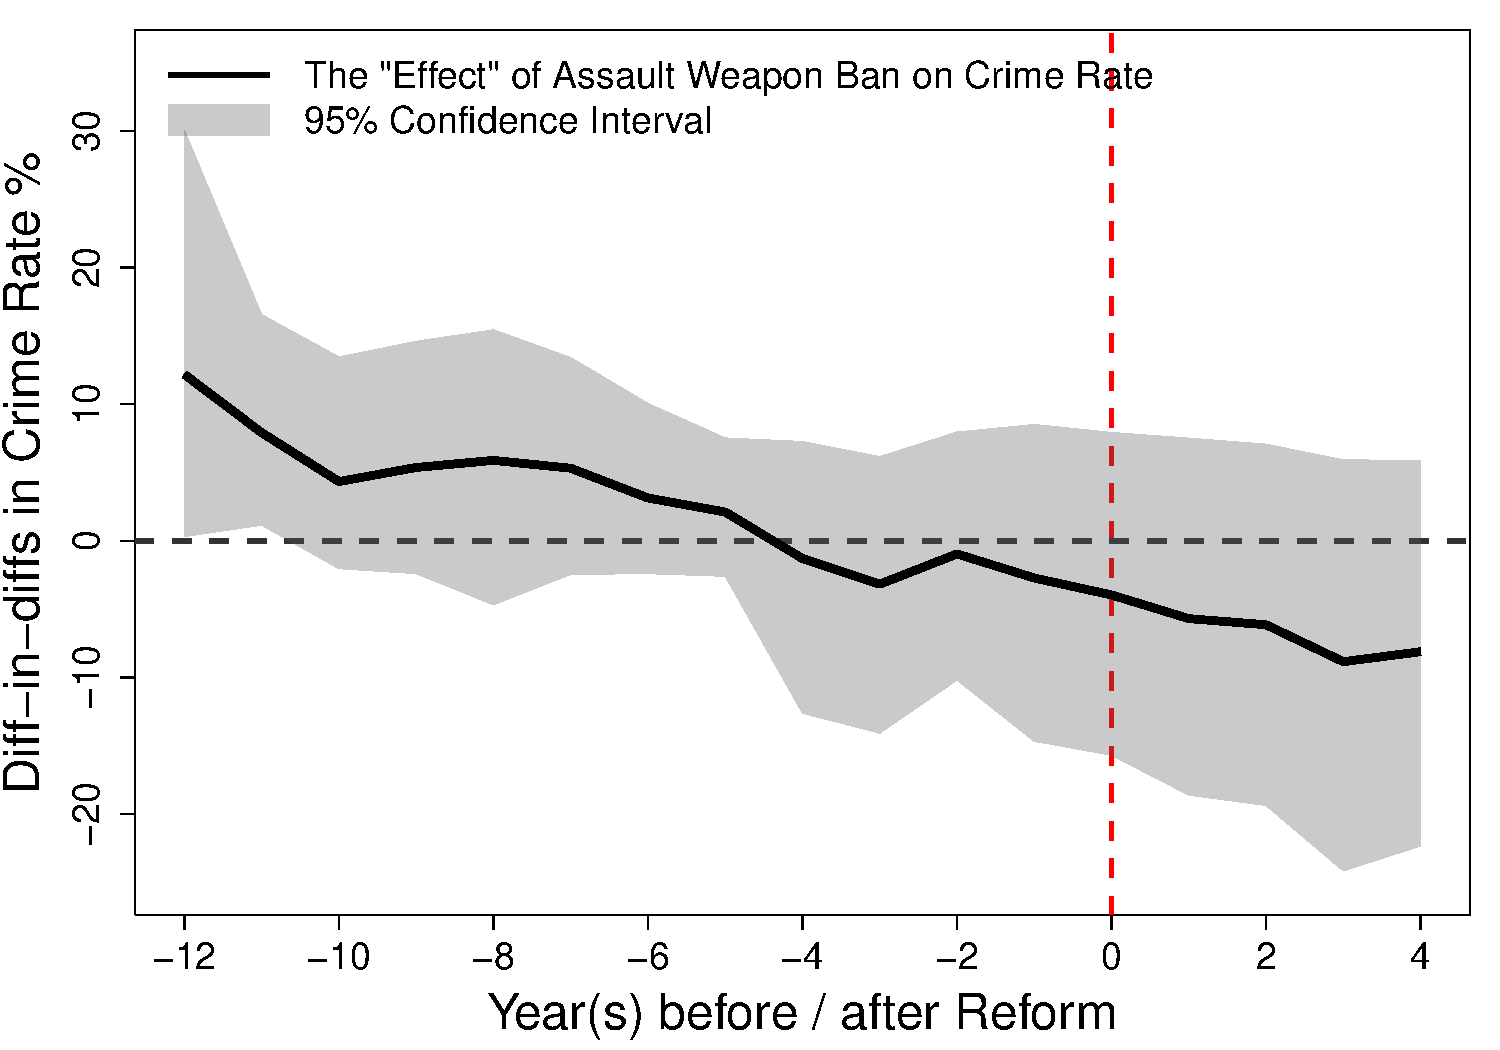
\includegraphics[width=\linewidth]{ex_guncontrol.pdf}
\end{column}
\begin{column}{0.49\textwidth}
\centering
\onslide<2->{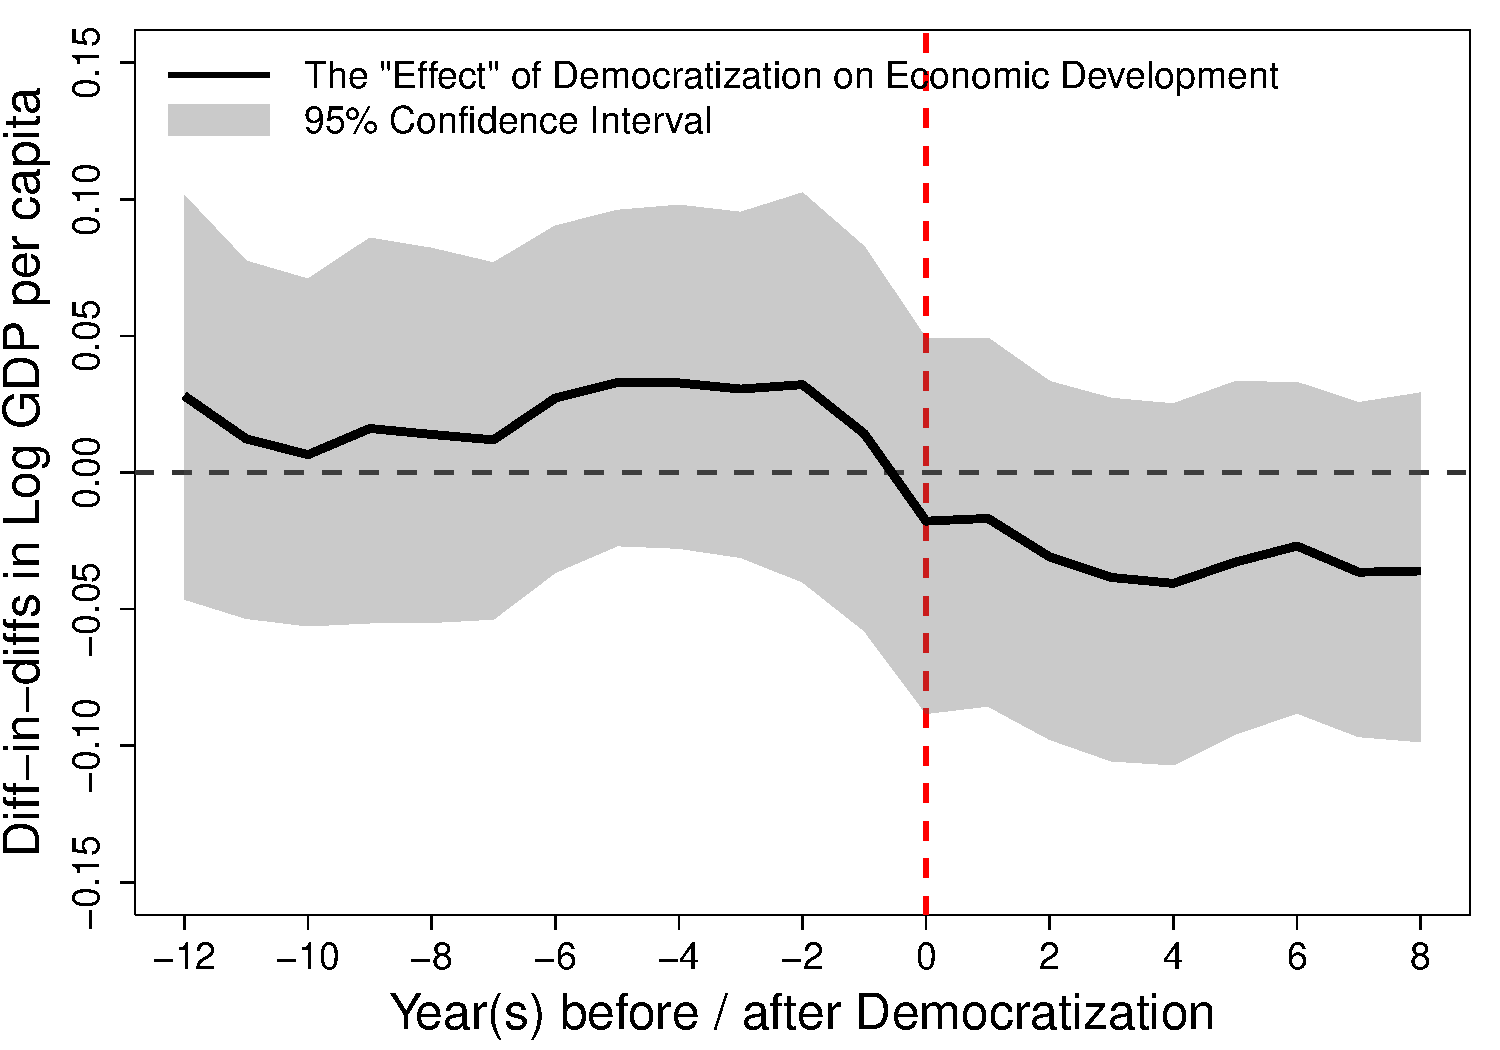
\includegraphics[width=\linewidth]{ex_demoGDP.pdf}}
\end{column}
\end{columns}
\bigskip
\begin{itemize}
\item<3-> Pre-treatment differences trend before the treatment ever arrives
\end{itemize}
\end{frame}

\begin{frame}
  \frametitle{Failure of Parallel Trends Is Common (2)}
\begin{columns}[T,onlytextwidth]
\begin{column}{0.49\textwidth}
\centering
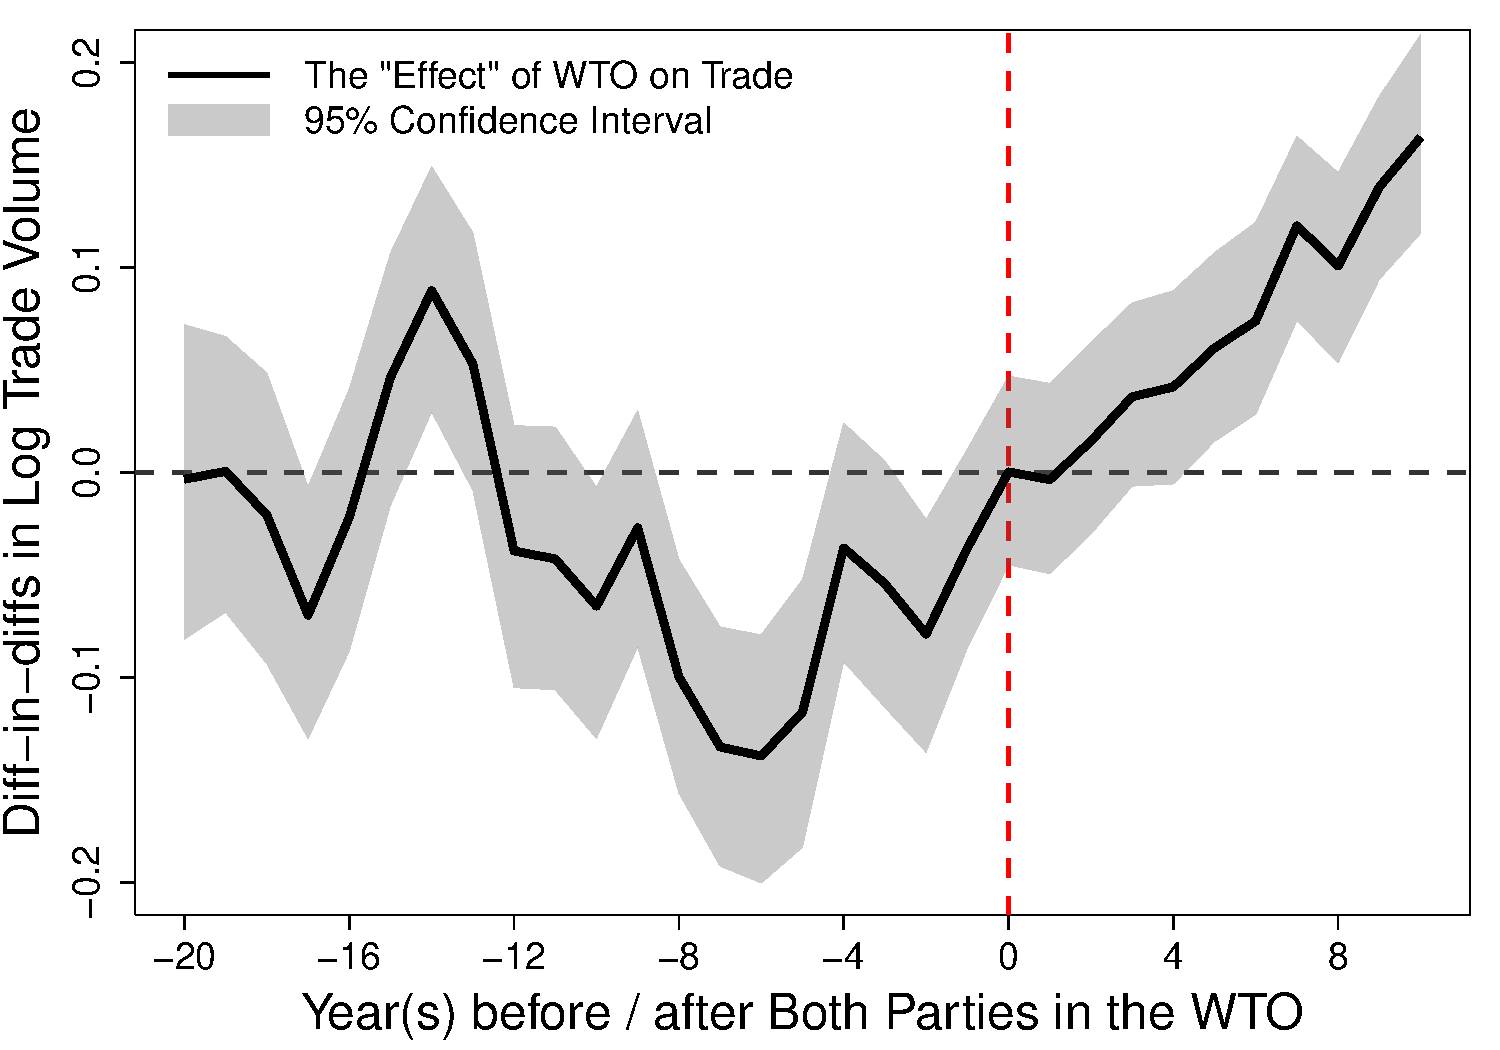
\includegraphics[width=\linewidth]{ex_trade.pdf}
\end{column}
\begin{column}{0.49\textwidth}
\centering
\onslide<2->{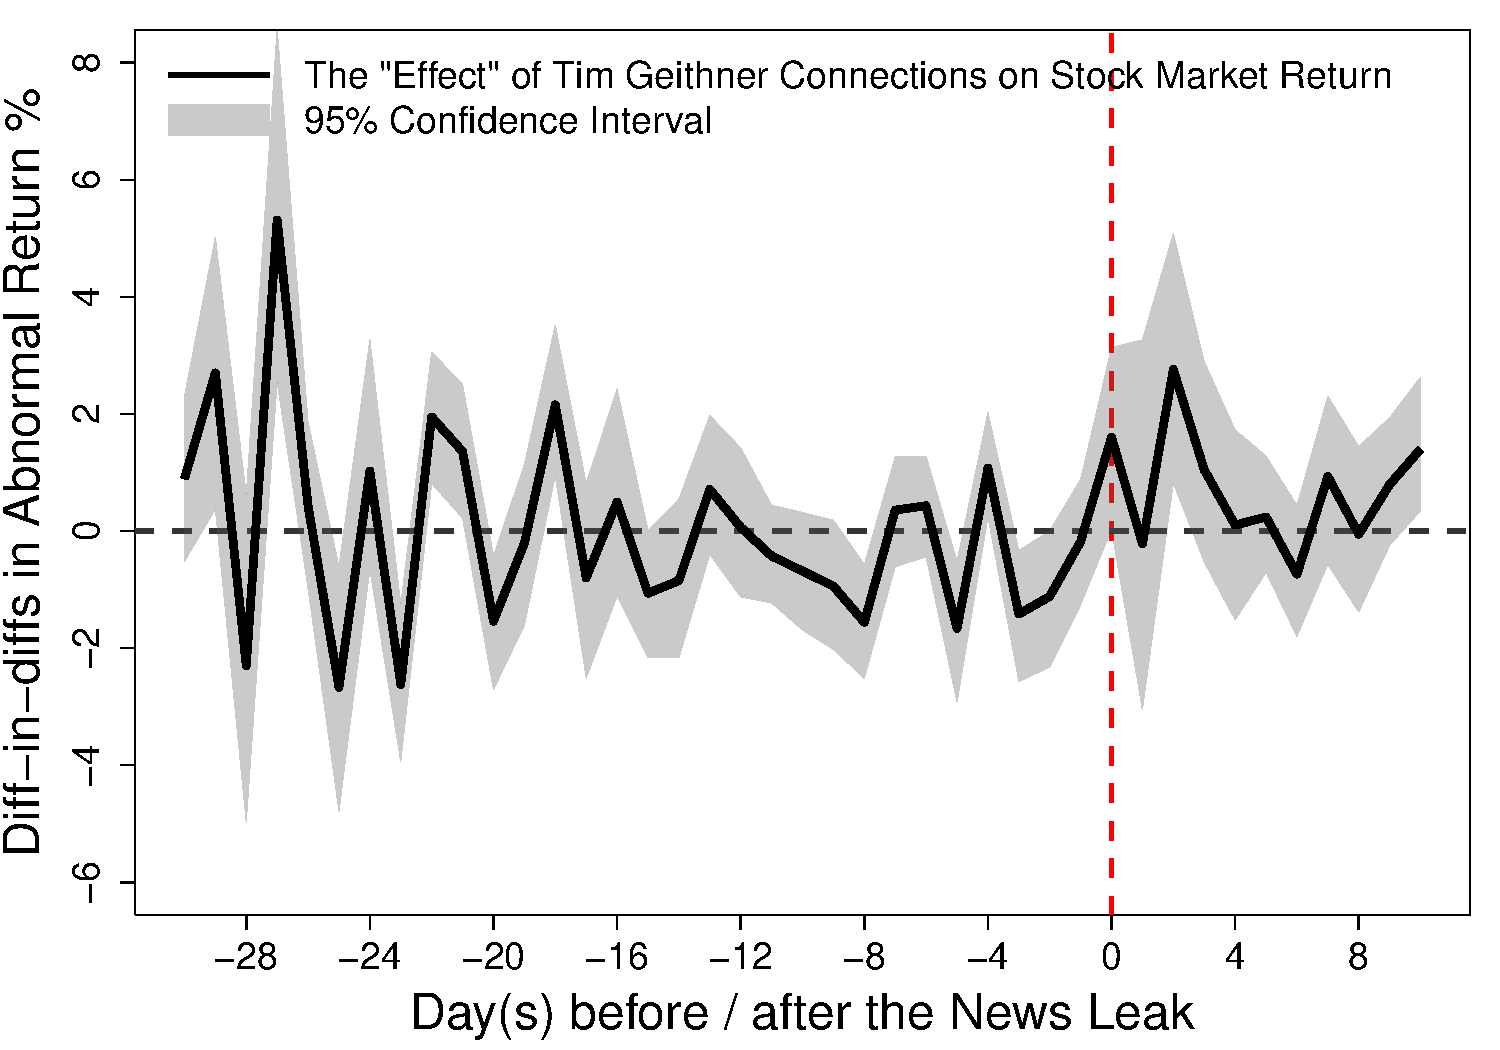
\includegraphics[width=\linewidth]{ex_ajkkm.pdf}}
\end{column}
\end{columns}
\bigskip
\begin{itemize}
\item<3-> Lesson: always plot the pre-treatment differences before interpreting the post-treatment ones
\end{itemize}
\end{frame}

\section{The Weighting Problem}

\begin{frame}
  \frametitle{What's the Weighting Problem?}
\begin{columns}[c]
\begin{column}{0.42\textwidth}
\begin{center}
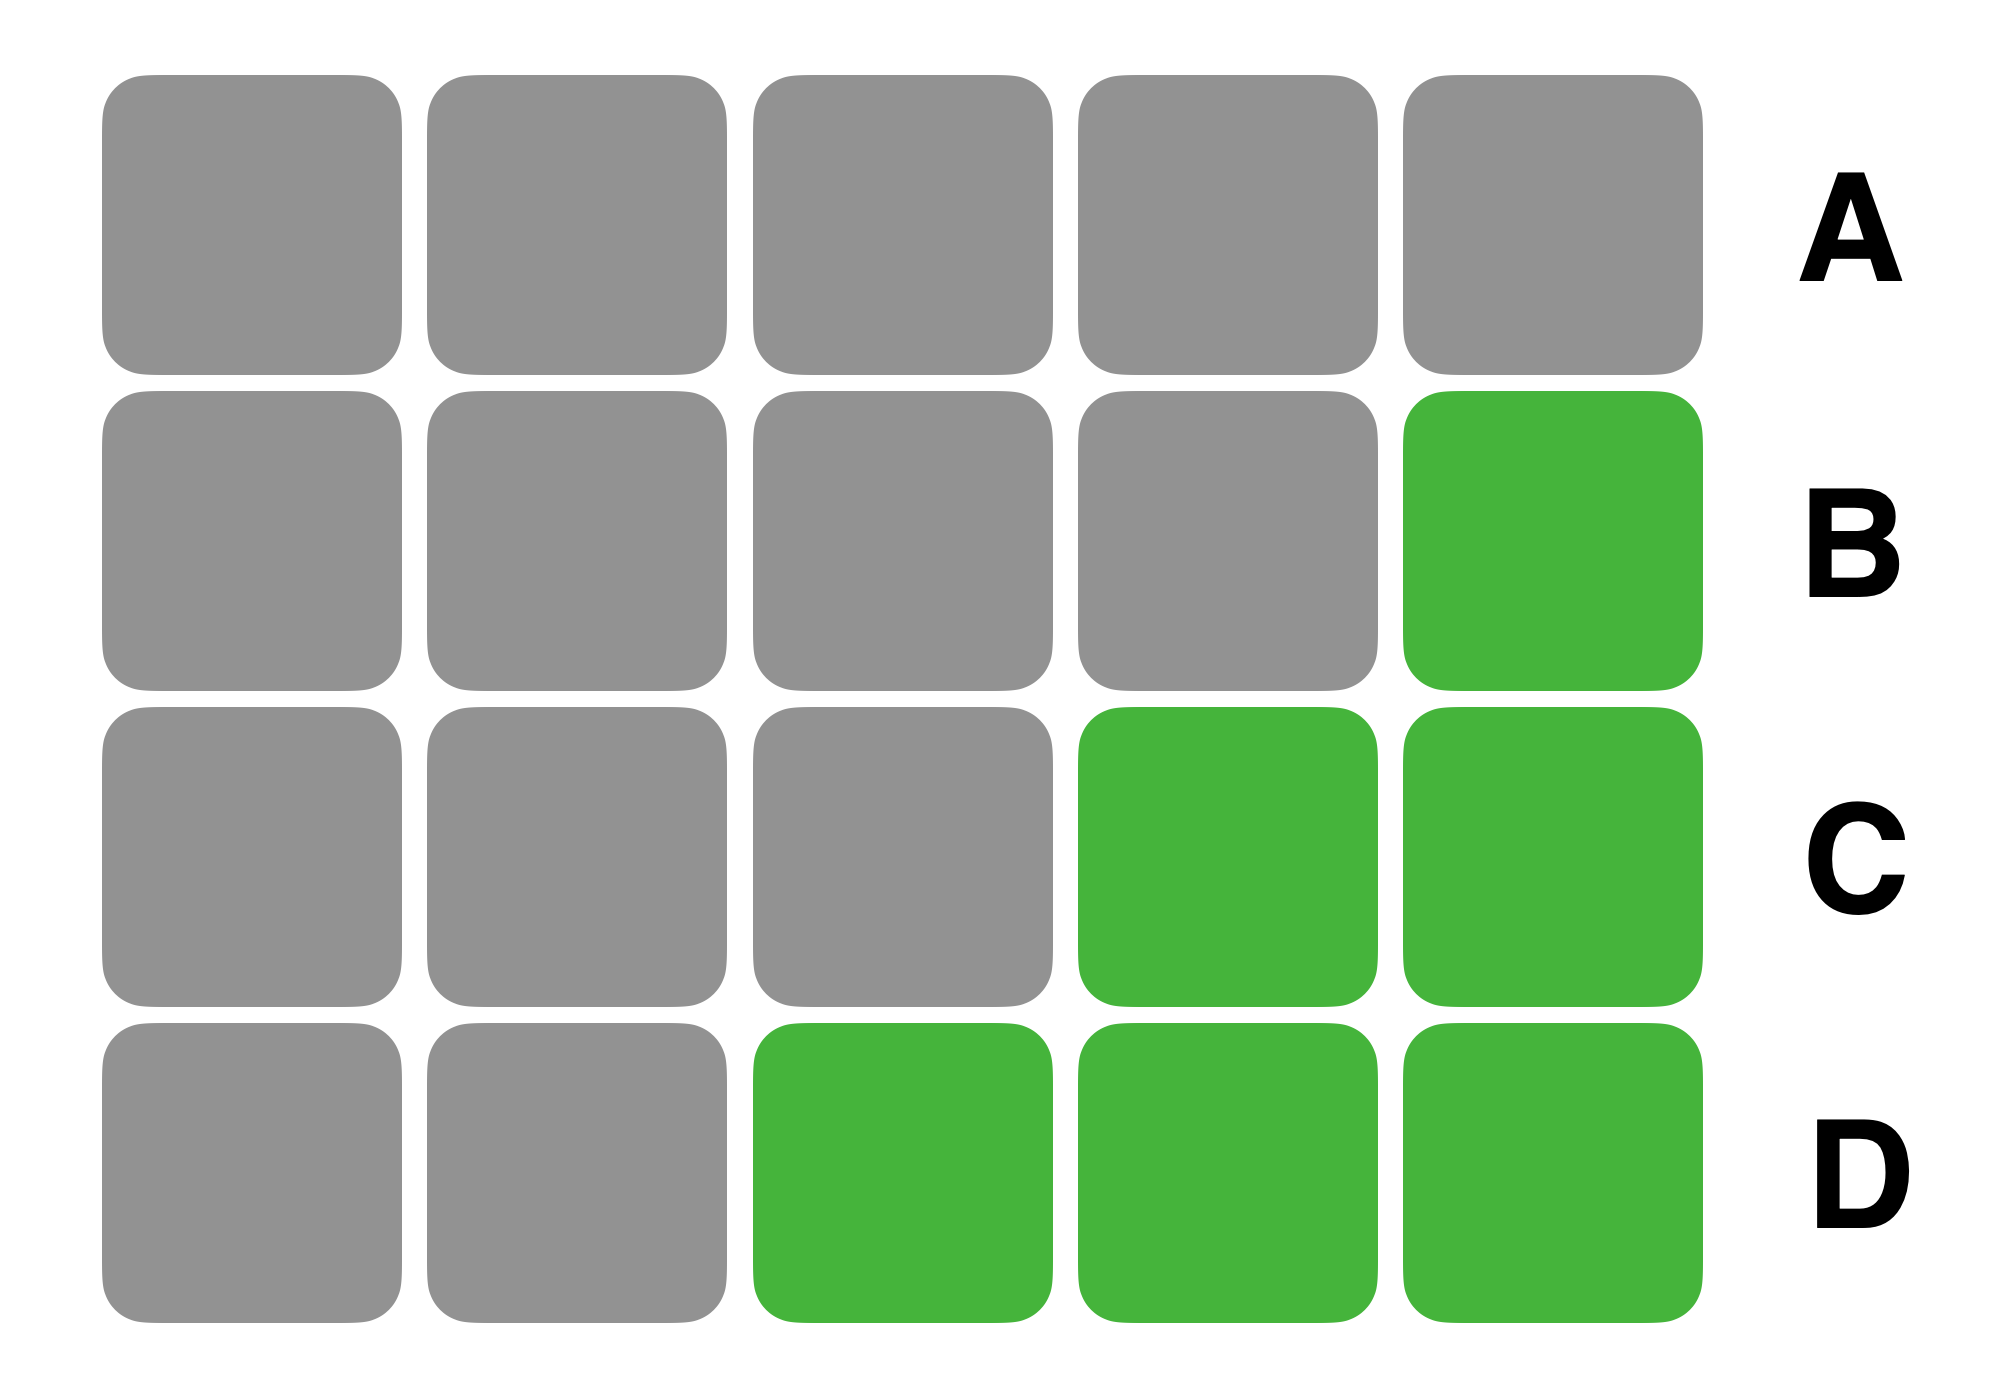
\includegraphics[width=\linewidth]{wordle.png}
\end{center}
\end{column}
\begin{column}{0.55\textwidth}
\begin{itemize}[<+->]\itemsep1em
\item Question: can TWFE recover (some \alert{non-negatively weighted}) ATT when treatment effects are heterogeneous?
\item Probably not! e.g. \alert{\textcite{goodman2021difference}, \textcite{dechaisemartin2020twoway}, \textcite{callaway2021difference}, \textciteshort{borusyak2021revisiting}, \textcite{strezhnev2018semiparametric}, \textcite{imai2021use}}
\item Early adopters (e.g. D) serve as comparisons for late adopters (e.g. B)
\item[$\Rightarrow$] Some \alert{treated} observations are used as comparisons
\end{itemize}
\end{column}
\end{columns}
\end{frame}

\begin{frame}
  \frametitle{\textcite{goodman2021difference}: TWFE Decomposition}
\begin{itemize}[<+->]\itemsep0.9em
\item Under staggered adoption, the TWFE estimator
\begin{equation*}
Y_{it} = \beta^{TWFE} D_{it} + \alpha_i + \xi_t + \varepsilon_{it}
\end{equation*}
is a \alert{weighted average of all possible $2\times 2$ DID estimators} that compare timing groups to each other
\item The weights are proportional to timing-group sizes and the variance of the treatment dummy in each pair, which is highest for units treated in the middle of the panel
\item Source of biases:
\begin{equation*}
\text{plim}_{N\rightarrow\infty}\, \hat{\beta}^{TWFE} = VWATT + VWCT - \Delta ATT
\end{equation*}
\begin{itemize}\itemsep0.4em
  \item $VWATT$: variance-weighted ATT
  \item $VWCT$: variance-weighted common trends
  \item $\Delta ATT$: change in treatment effects over time
\end{itemize}
\end{itemize}
\end{frame}

\begin{frame}
  \frametitle{The Three-Group Case}
\begin{columns}[c]
\begin{column}{0.4\textwidth}
\begin{itemize}\itemsep1em
\item An early group $k$, treated at $t_i = k$
\item A late group $\ell$, treated at $t_i = \ell > k$
\item An untreated group $U$, $t_i = \infty$
\end{itemize}
\end{column}
\begin{column}{0.58\textwidth}
\begin{center}
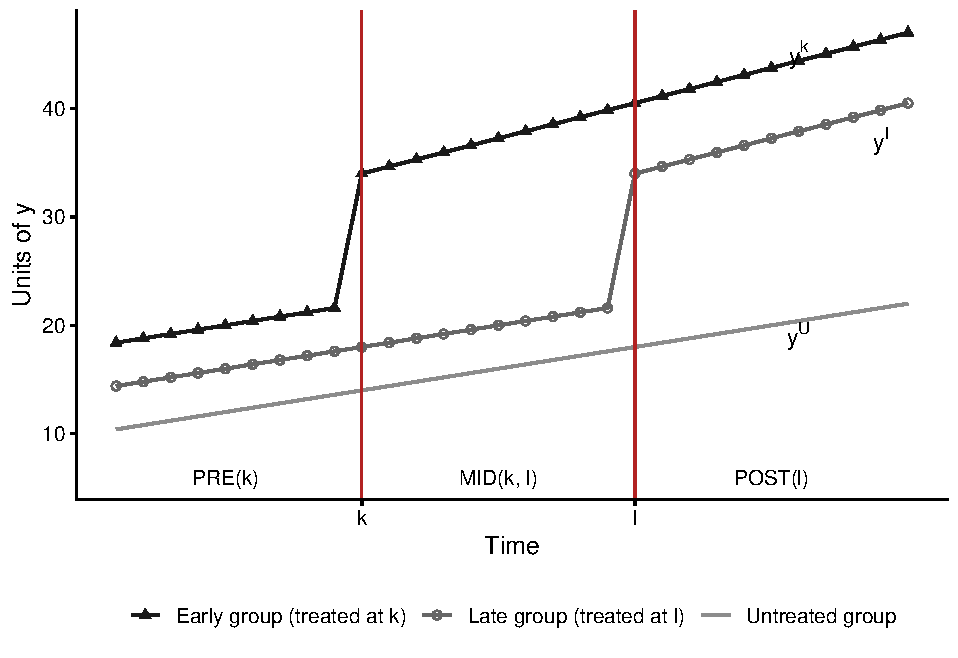
\includegraphics[width=\linewidth]{gb_threegroups_2026.pdf}
\end{center}
\end{column}
\end{columns}
\slidesource{Redrawn after \textcite{goodman2021difference}, Figure 1 (\texttt{goodman\_bacon\_2026.R}).}
\end{frame}

\begin{frame}
  \frametitle{Four Simple ($2\times 2$) DID Estimates}
\begin{center}
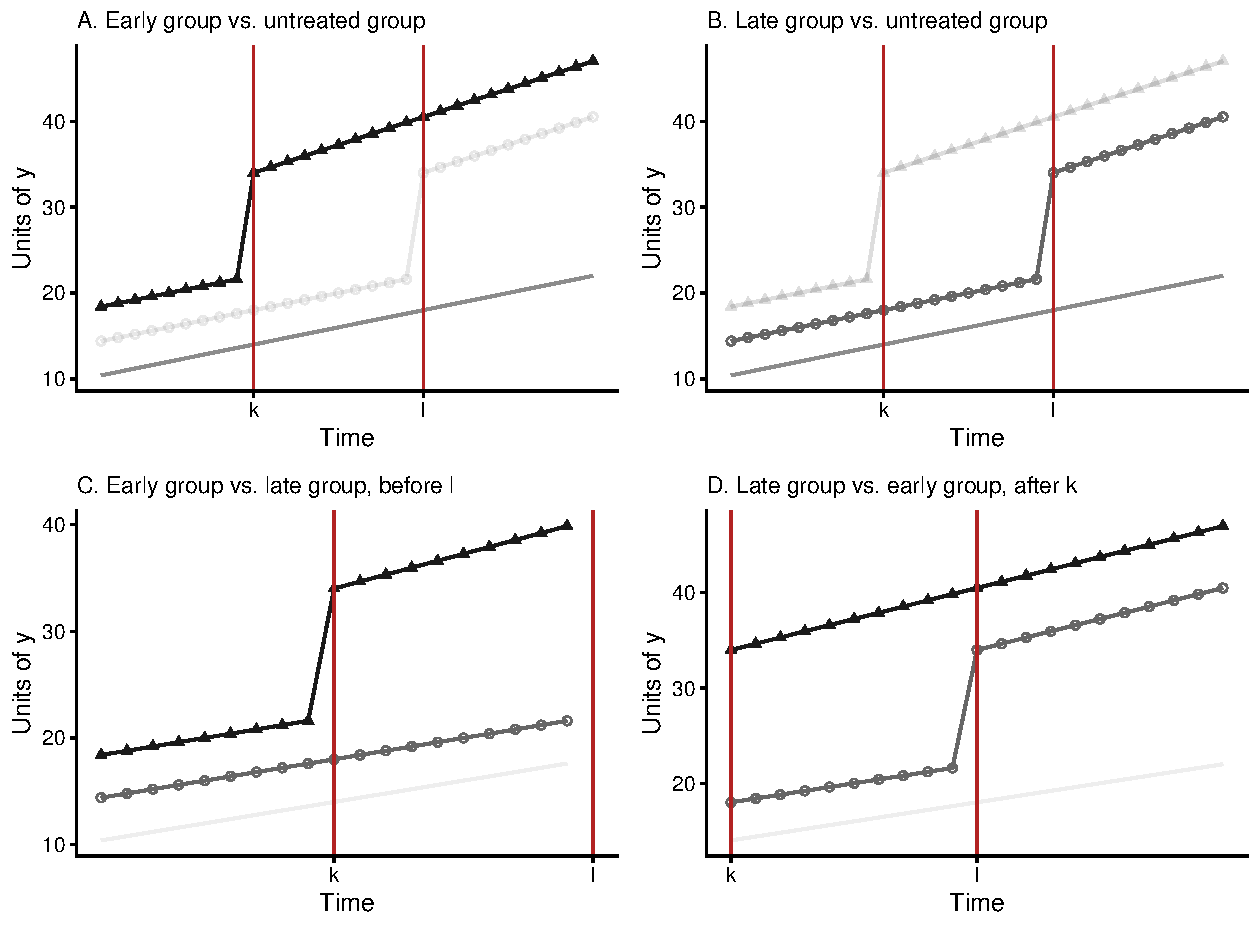
\includegraphics[height=0.6\textheight]{gb_four2x2_2026.pdf}
\end{center}
\begin{itemize}
\item<2-> Panel D is the troublemaker: the \alert{already-treated} early group serves as the comparison, and its evolving treatment effect enters with a \alert{negative sign}
\end{itemize}
\slidesource{\textcite{goodman2021difference}.}
\end{frame}

\begin{frame}
  \frametitle{Example: No-Fault Divorce Reforms and Female Suicide}
\begin{itemize}
\item 37 states adopted unilateral divorce between 1969 and 1985 (9 had reformed before 1964, 5 never did); event-study and TWFE estimates:
\end{itemize}
\begin{center}
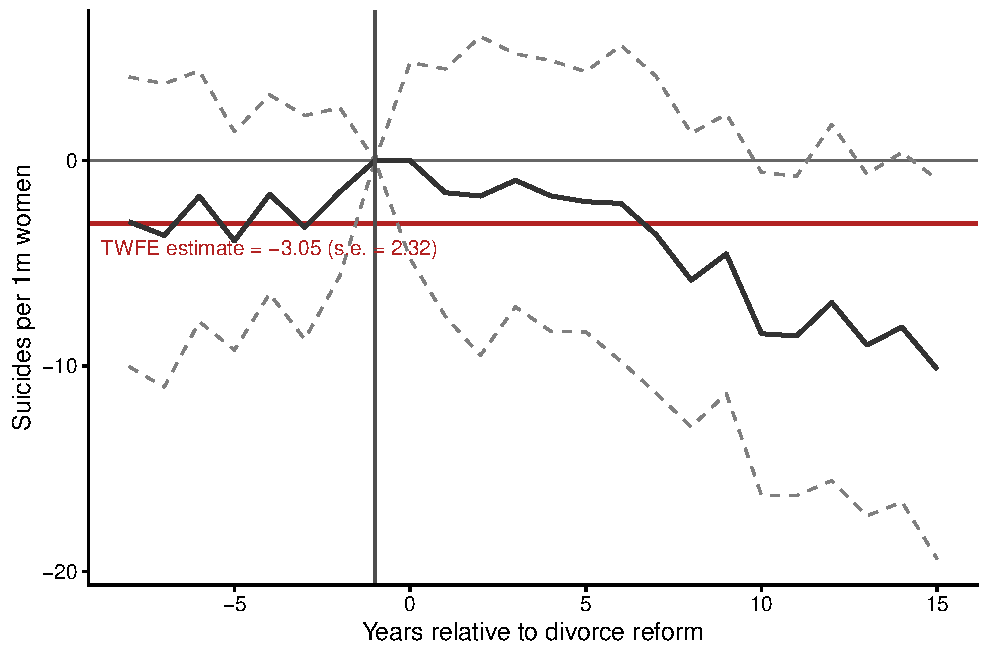
\includegraphics[height=0.66\textheight]{gb_divorce_es_2026.pdf}
\end{center}
\slidesource{Own replication of the divorce example in \textcite{goodman2021difference}; Stevenson and Wolfers (2006) data from the \texttt{bacondecomp} package (\texttt{goodman\_bacon\_2026.R}).}
\end{frame}

\begin{frame}
  \frametitle{Decomposing the Divorce Estimate}
\begin{itemize}
\item Plot each $2\times 2$ DID against its weight; average effect and total weight by comparison type:
\end{itemize}
\begin{center}
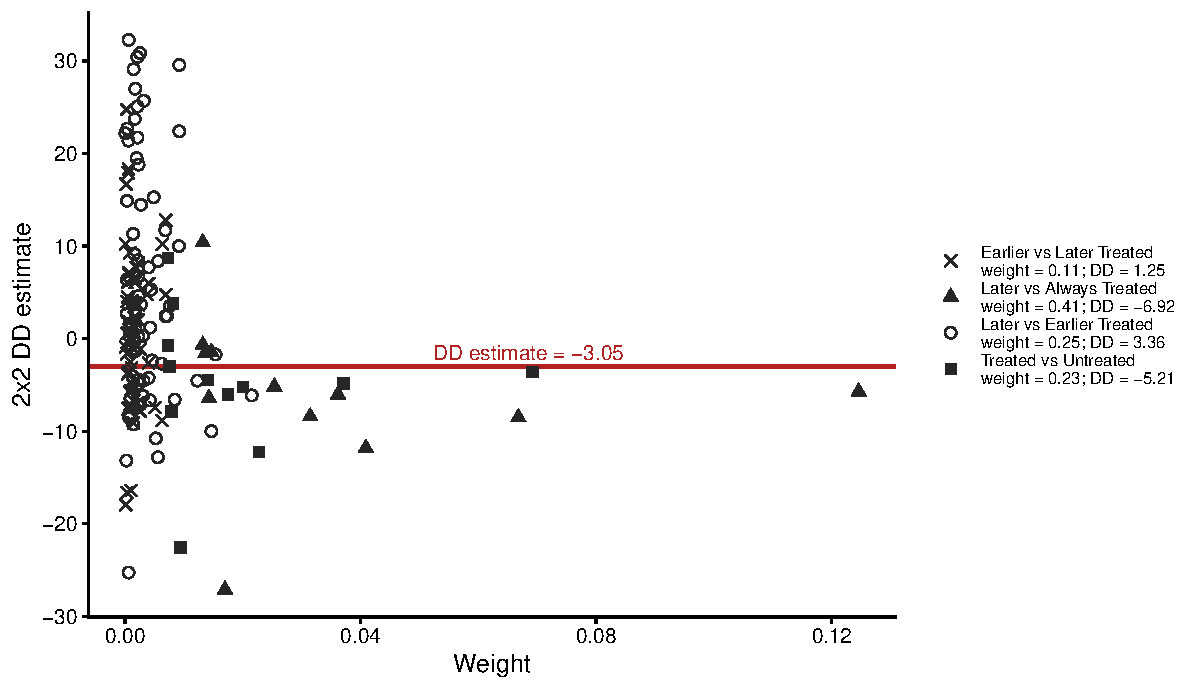
\includegraphics[height=0.6\textheight]{gb_weights_2026.pdf}
\end{center}
\begin{itemize}
\item<2-> The TWFE estimate, $-3.05$ (Goodman-Bacon reports $-3.08$), is the average of the $y$-axis values weighted by the $x$-axis values
\end{itemize}
\slidesource{Own replication with the \texttt{bacondecomp} package (\texttt{goodman\_bacon\_2026.R}).}
\end{frame}

\begin{frame}
  \frametitle{Negative Weights (\cite{dechaisemartin2020twoway})}
\begin{itemize}[<+->]\itemsep1em
\item A complementary result: under heterogeneous effects, the TWFE coefficient satisfies
\begin{equation*}
\hat{\beta}^{TWFE} \;\xrightarrow{p}\; \E\Big[\sum_{(i,t):\, D_{it}=1} w_{it}\, \tau_{it}\Big]
\end{equation*}
where the weights $w_{it}$ sum to one but \alert{some can be negative}
\item Negative weights attach to observations treated for a long time in periods when many units are treated
\item With negative weights, $\hat{\beta}^{TWFE}$ can be negative even if every $\tau_{it} > 0$: a \alert{sign reversal}
\item Diagnostic: the \texttt{twowayfeweights} package reports the share and sum of negative weights for your design
\end{itemize}
\end{frame}

\begin{frame}
  \frametitle{Event-Study TWFE Is Not Safe Either (\cite{sun2021estimating})}
\begin{itemize}[<+->]\itemsep1.2em
\item The same logic contaminates the dynamic specification: each lead or lag coefficient $\hat{\mu}_s$ is a weighted average that picks up effects from \alert{other relative periods} and \alert{other cohorts}
\item In particular, lead coefficients can appear non-zero even when parallel trends holds, and can appear zero when it fails
\item So under staggered adoption with HTE, the standard event-study plot is not a reliable pre-trend diagnostic
\item Fix: estimate cohort-specific effects and aggregate them explicitly, e.g. the interaction-weighted estimator (Lecture 5)
\end{itemize}
\end{frame}

\begin{frame}
  \frametitle{How Bad Is the Weighting Problem in Practice? (\citeshort{chiu2026causal})}
\begin{columns}[c]
\column{.4\textwidth}
\vspace{-2em}
\begin{itemize}[<+->]\itemsep1em
\item Not too bad!
\item Reanalyzing published studies from top political science journals, we find:\medskip
\begin{itemize}[<+->]\itemsep0.5em
\item There is almost no sign flipping
\item No systematic overestimation or underestimation of the treatment effects
\item Some marginally significant results become insignificant
\item However, parallel trends violations remain a major concern
\end{itemize}
\item Lecture 5 returns to this study in detail
\end{itemize}\pause
\column{.6\textwidth}
\begin{center}
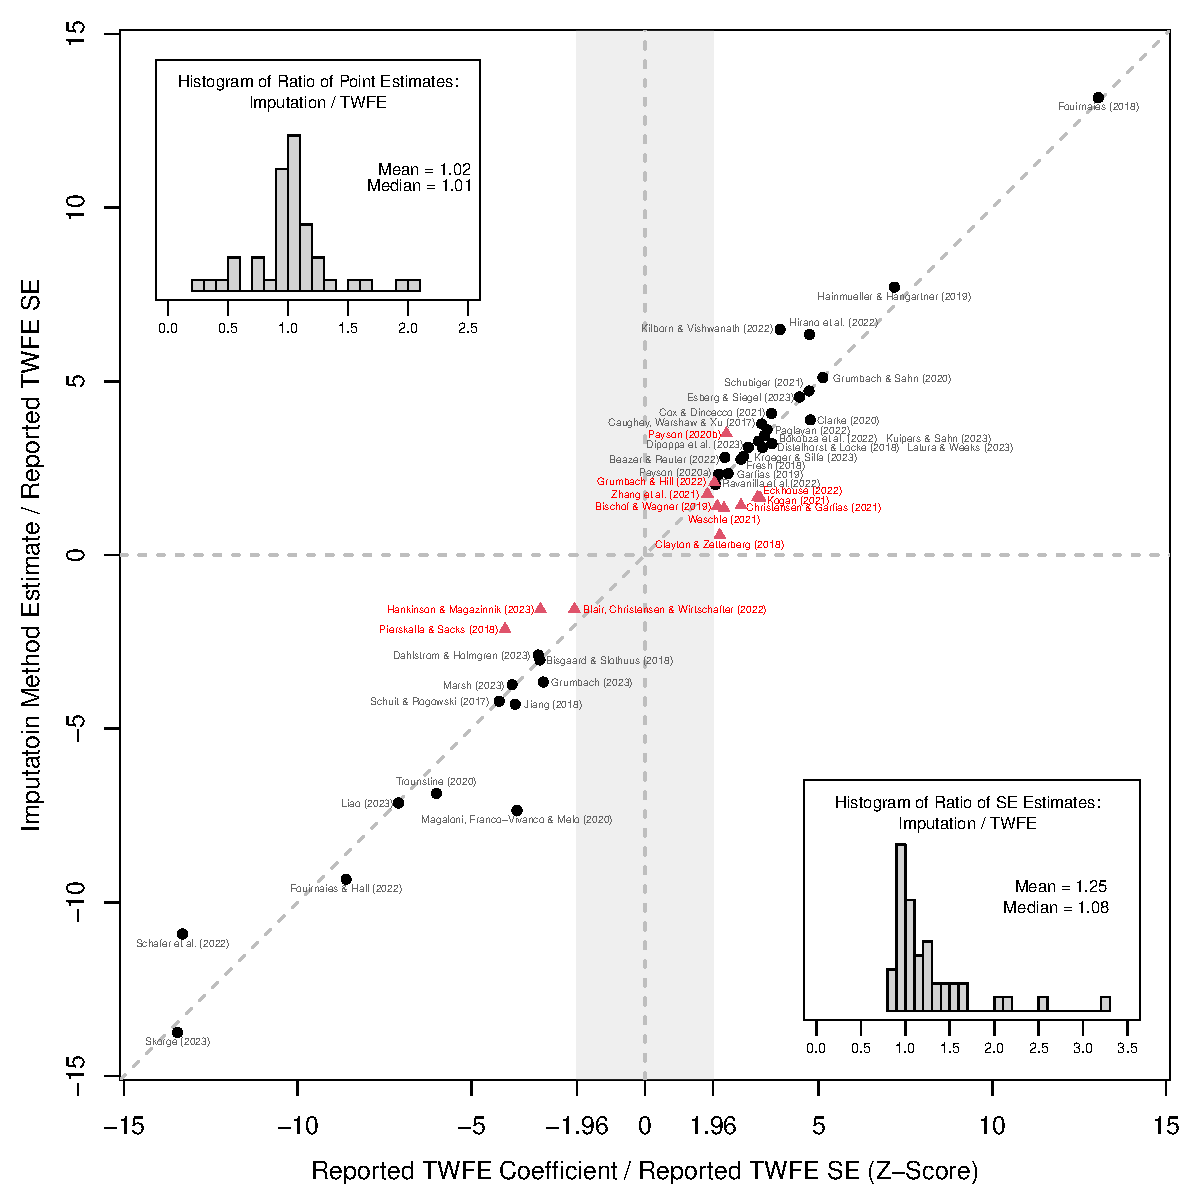
\includegraphics[width=\textwidth, height=0.8\textheight, keepaspectratio]{fig3_est_all.pdf}%
\end{center}
\end{columns}
\end{frame}

\begin{frame}
  \frametitle{Taking Stock}
\begin{itemize}[<+->]\itemsep1.2em
\item TWFE on staggered data mixes clean and contaminated comparisons; with heterogeneous effects, the estimand is no longer any ATT we care about
\item In practice, the first-order threat is usually \alert{parallel trends failure}, not the weighting problem itself
\item Both problems have the same root: the regression does not distinguish \emph{which} observations serve as comparisons for \emph{which} treated observations
\item The fix: make the comparisons explicit, which is what the modern estimators do
\item[$\Rightarrow$] The road ahead: Lecture 5 repairs the \alert{weighting problem}; Lecture 6 introduces low-rank methods that can address \alert{some} parallel trends violations.
\end{itemize}
\end{frame}

\begin{frame}
  \frametitle{Addressing Potential Parallel Trends Violations}
\begin{itemize}[<+->]\itemsep0.9em
\item \textbf{Condition on pre-treatment covariates}: parallel trends holds within strata of $X$
\begin{itemize}\itemsep0.4em
  \item Semiparametric DID, e.g. \alert{\textcite{abadie2005semiparametric}; \textcite{callaway2021difference}} $\rightarrow$ Lecture 5
\end{itemize}
\item \textbf{Condition on pre-treatment outcomes}: build the comparison from units whose pre-trends match
\begin{itemize}\itemsep0.4em
  \item Synthetic control, e.g. \alert{\citeauthorshort{abadie2010synthetic} (\citeyear{abadie2010synthetic}, \citeyear{abadie2015comparative})} $\rightarrow$ Lecture 6
\end{itemize}
\item \textbf{Model the confounding}: impute $Y_{it}(0)$ from a low-rank (latent factor) model fit on untreated data
\begin{itemize}\itemsep0.4em
  \item \alert{\textcite{gobillon2016regional}; \textcite{xu2017generalized}; \textcite{athey2021matrix}} $\rightarrow$ Lecture 6
\end{itemize}
\item \textbf{Combine weighting and modeling}: doubly robust hybrids
\begin{itemize}\itemsep0.4em
  \item Augmented synthetic control (\alert{\citeshort{benmichael2021augmented}}); synthetic DID (\alert{\cite{arkhangelsky2021synthetic}}) $\rightarrow$ Lecture 6
\end{itemize}
\end{itemize}
\end{frame}


\section{Conclusions}

\begin{frame}
  \frametitle{Summary}
\begin{itemize}[<+->]\itemsep1.2em
\item TWFE models require stronger assumptions than we normally admit; both treatment effect heterogeneity and parallel trends failures can lead to bias
\item Under staggered adoption, TWFE averages all $2\times 2$ comparisons, including ones that use already-treated units as comparisons
\item In reanalyses of published work, the weighting bias is usually modest; parallel trends violations are the bigger threat
\item Current solutions: matching/reweighting, imputation, and their combinations
\item Whichever method you use, run the diagnostics: plot the pre-trend and run placebo tests. They can reject parallel trends, but they cannot prove it.
\end{itemize}
\end{frame}

\begin{frame}
  \frametitle{Software}
\begin{itemize}\itemsep0.5em
\item \texttt{fixest}: fast fixed effects regressions
\item \texttt{bacondecomp}: Goodman-Bacon decomposition
\item \texttt{did}: Callaway and Sant'Anna's estimator
\item \texttt{PanelMatch}: panel matching
\item \texttt{fect}: imputation estimators (FEct, IFEct, MC) with diagnostic tests
\item \texttt{gsynth}: interactive fixed effects with non-reversible treatments
\item \texttt{panelView}: panel data visualization
\end{itemize}
\bigskip
Lectures 5 and 6 demonstrate several of these in worked examples.
\end{frame}

\appendix

\setbeamertemplate{frametitle continuation}[from second][(cont.)]
\begin{frame}[t,allowframebreaks=1.0]
  \frametitle{References}
  \referencelist
\end{frame}


\end{document}
